\section{Slide Example}
\label{ASlideExample}
The test code for NISSE in ''Time Efficiency Test'' in section \ref{TimeEfficiencyTest} is shown in listing \ref{NISSETest}.
The test slides contains a variation of elements, that can be expressed in NISSE.
Figure \ref{fig:EfficiencyTest} shows the output of the listing \ref{NISSETest}.

\begin{lstlisting}[frame=single,caption=Time Efficiency Test code for NISSE, label=NISSETest]
@begin{slide}
@title{Frontpage}
@subtitle{d. 07-05-2012}
@end{slide}

@begin{slide}
    @title{Lecture 1}
    
    This is lecture 1 of 10 lectures in programming languages
    The basic elements are:
*Loop
*Functiones
*if statements
@end{slide}

@begin{slide}
    Later in this course you will laern how to create pictures. This is a blck picture.
    @image{@url:http://freeimagesarchive.com/data/media/3/2_black.jpg | http://media.desura.com/images/members/1/288/287053/black_1.2.jpg}
@end{slide}

@begin{slide}
    We also have a lot of @b{breaks} in this course.
    We will have a coffee break until the end.
@end{slide}

@begin{slide}
    @title{Next lecture}
    @subtitle{On 15.05.2012}
    
    This was all for now.
    Have a nice day.
    The curent slideshow can be found at @apply{@url:http://www.somelink.com | this link }.
@end{slide}

\end{lstlisting}


\begin{figure}[htbp]
	\centering
		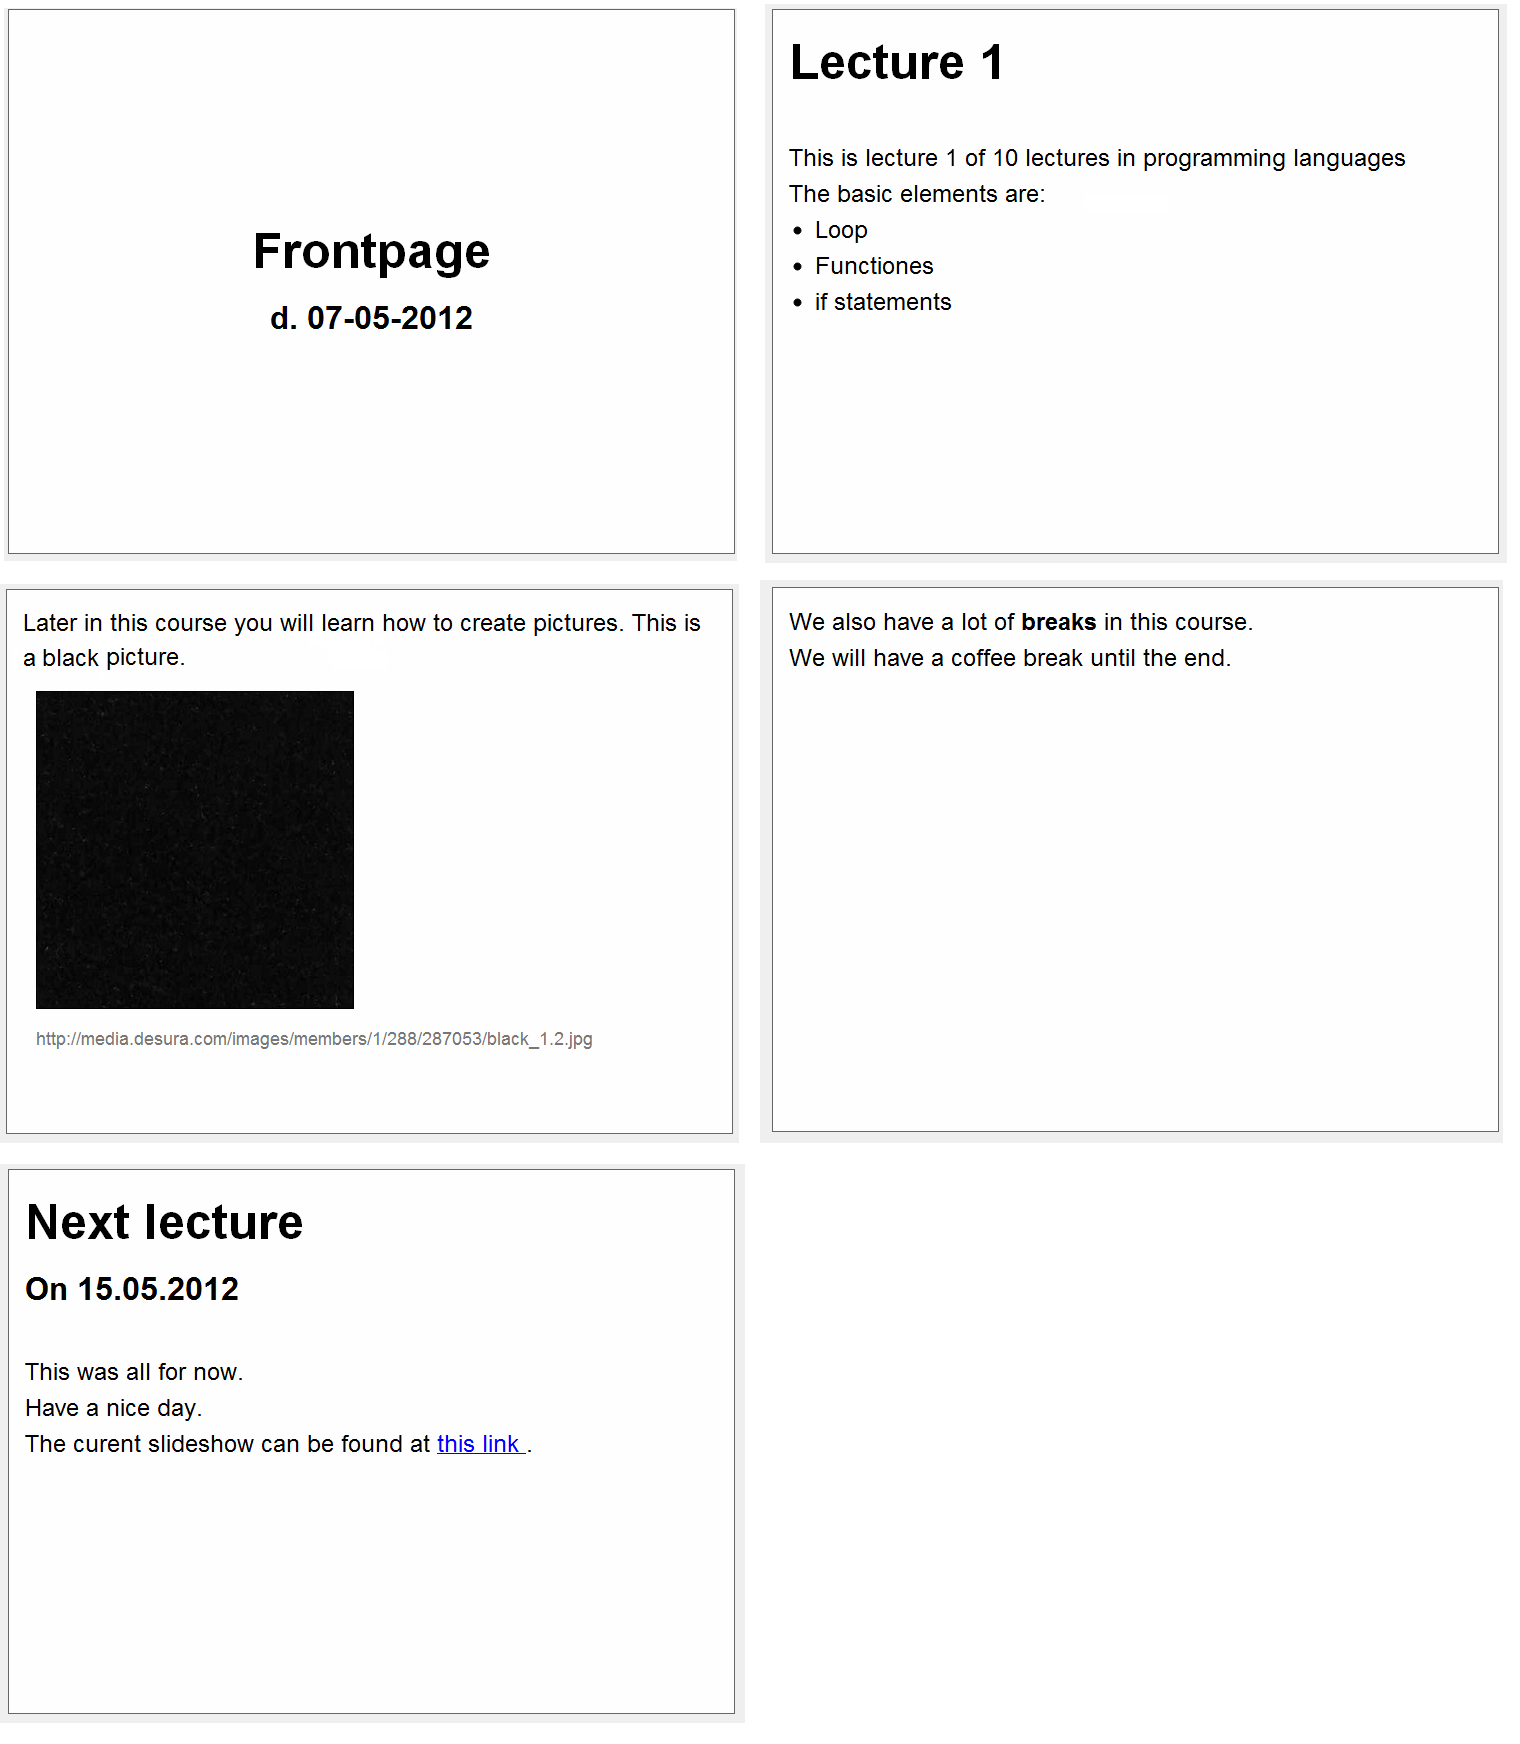
\includegraphics[width=1.00\textwidth]{./images/EfficiencyTest.png}
	\caption{Output of the code}
	\label{fig:EfficiencyTest}
\end{figure}

